% Nama Kelompok : 
% Kelas : D4 TI 1A
% Anggota : 
% 1. Harun    1174027
% 2. Fahmi    1174021
% 3. Kukuh    1174016
% 4. Izzah    1174013
% 5. Rizal    1174014
% 6. Lawimner 1174030





Artikel tentang informasi mengenai RAM

  \begin{figuress}[ht]
  \centerline{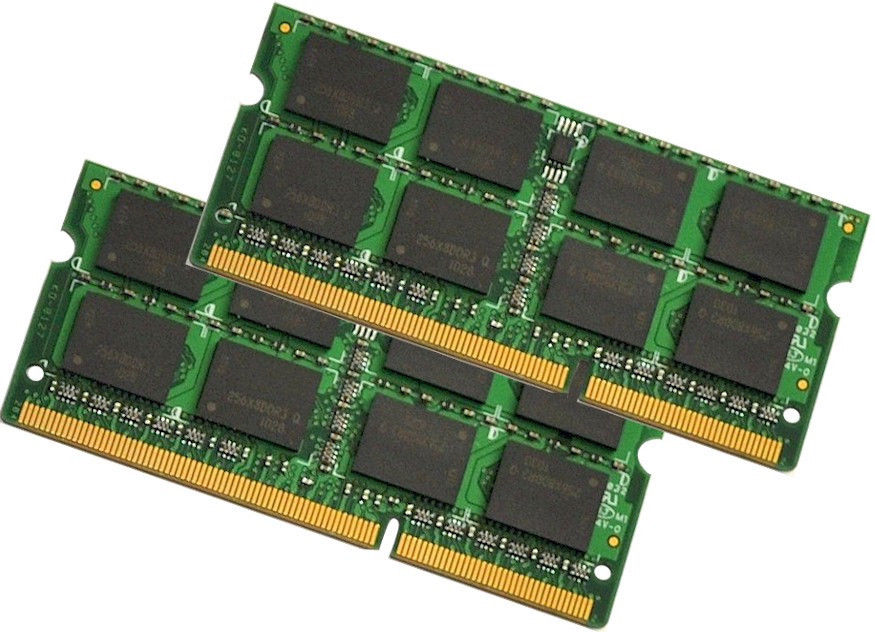
\includegraphics[width=1\textwidth]{figuress/RAM.jpg}}
  \caption{Pengertian RAM}
  \label{RAM}
  \end{figuress}

\section{Pengertian RAM}
Gambar RAM \ref{RAM}
RAM kepanjangan dari Random Access Memory yang biasa terdapat di HP,di Komputer dan di leptop.
RAM adalah sebuah tipe penyimpanan komputer yang isinya dapat diakses dalam waktu yang tetap tidak mempedulikan letak data tersebut dalam memori.
RAM juga bisa menjadi tempat penyimpanan data,tapi hal ini hanya bersifat sementara saja.
RAM atau Random Acces Memory sebagai Memori Utama . Ram juga penentu seberapa cepat PC menjalankan Aplikasi.
RAM biasanya berukuran 128 mb 256 mb 512 mb 1 gb 2 gb 4 gb 8 gb 16 gb.

\section{Fungsi RAM}
Fungsi RAM adalah untuk mempercepat pemprosesan data pada PC/Komputer. Semakin besarnya RAM yang dimiliki, semakin cepatl pula komputer tersebut.
Selain itu, RAM juga berfungsi sebagai mendia penyimpanan disaat komputer atau laptop dalam keadaan hidup, apabila laptop atau komputer dimatikan maka data yang tersimpan dalam ram akan hilang dan terhapus. Misalkan disaat kita mengetik dokumen di microsoft word kemudian kita tutup tanpa klik save, data yang anda ketik akan tersimpan di memori ram, dengan begitu anda dapat membuka dokumen tersebut melalui history terakhir atau melalui auto save.

\section{Struktur ram}
RAM juga memiliki 4 struktur utama yaitu :
Yang petama yaitu Input storage yang memiliki fungsi untuk menampung input yang dimasukkan melalui alat input.
Yang kedua yaitu Program storage Yang memiliki fungsi untuk menyimpan semua instruksi\-instruksi program yang akan diakses.
Yang ketiga yaitu Working storage Yang memiliki fungsi untuk menyimpan data yang akan diolah dan hasil pengolahan.
Yang Terakhir yaitu Output storage Yang memiliki fungsi untuk menampung hasil akhir dari pengolahan data yang akan ditampilkan ke alat output.

\section{Sejarah RAM}
Random Acces Memory atau biasa di sebut RAM di temukan oleh Robert Dennard.
Pertama kali dikenal pada tahun 60′an. Hanya saja saat itu memori semikonduktor belumlah populer karena harganya yang sangat mahal. Saat itu lebih lazim untuk menggunakan memori utama magnetic. Perusahaan semikonduktor seperti Intel memulai debutnya dengan memproduksi RAM, lebih tepatnya jenis DRAM. 
Perkembangan Random Access Memory(RAM) sangatlah cepat sehingga beberapa ahli komputer pun turut berpartisipasi untuk melakukan pengklasifikasian dalam evolusi RAM ini. 
Berikut perkembangan RAM dari masa ke masa, diantaranya:

1.  RAM (Random Access Memory). Ditemukan oleh Robert Dennard dan diproduksi secara besar\-besaran oleh perusahaan Intel pada tahun 1968, jauh sebelum komputer ditemukan oleh IBM pada tahun 1981. Dari sinilah awal perkembangan RAM bermula. Pada saat awal pembuatannya, RAM ini membutuhkan tegangan kerja setidaknya sebesar 5.0 volt agar bisa bekerja secara optimal pada frekuensi 4,77MHz, dan membutuhkan waktu akses memori (access time) yang cukup besar kurang lebih sekitar 200ns, 1ns itu sama seperti 10\-9 detik,jadi membutuhkan 2000 detik untuk mengolah data.

2.  DRAM.(Dynamic Random Access Memory) Pada tahun 1970, IBM membuat sebuah memori yang dinamakan DRAM yang merupakan kepanjangan Dynamic Random Access Memory. Dari diberi nama Dynamic bukan berati hanya pemberian nama, tapi karena memori ini bekerja pada interval waktu tertentu, yang sifatnya selalu memperbarui keakuratan informasi atau isinya. DRAM mempunyai frekuensi kerja yang cukup bervariasi, yaitu antara 4,77MHz sampai 40MHz. 

3.  FPM RAM. Fast Page Mode Dynamic Random Access Memoery atau disingkat dengan FPM DRAM ditemukan sekitar tahun 1987 atau yang lebih sering di kenal dengan nama FPM. FPM ini bisa melakukan transfer data yang lebih cepat pada baris (row) yang sama dari jenis memori sebelumnya yaitu DRAM. FPM RAM ini bekerja pada frekuensi mulai dari 16MHz sampai 66MHz dengan membutuhkan access time sekitar 50ns atau 500 detik. Selain itu juga FPM RAM ini mampu melakukan transfering data (bandwidth) sebesar 188,71 MegaBytes (MB) per detiknya.

4.  EDO RAM.(Extended Data Output Dynamic Random Access Memory) Pada tahun 1995, dibuatlah memori jenis Extended Data Output Dynamic Random Access Memory (EDO DRAM) yang merupakan penyempurnaan dari FPM. Memori EDO dapat mempersingkat lingkaran membacanya sehingga dapat meningkatkan kinerjanya sekitar 20\%. EDO mempunyai access time yang bermacam macam, mulai dari 70ns hingga 50ns dan bekerja  pada frekuensi 33MHz hingga 75MHz. Meskipun EDO RAM merupakan memoeri yang disempurnakan dari FPM RAM, tetapi keduanya RAM tidak dapat dipasangkan secara bersamaan, karena adanya perbedaan kemampuan kinerja pada kedua RAM ini. EDO DRAM sepertinya banyak digunakan pada sistem yang berbasis Intel 486 dan kompatibel dengan intel Pentium generasi awal.

5.  SDRAM PC66.(Synchronous Dynamic Random Access Memory) Pada awal tahun 1996 hingga akhir 1997 Menemukan Synchronous Dynamic Random Access Memory atau disingkat SDRAM. SDRAM ini kemudian jauh lebih dikenal dengan sebutan PC66 karena RAM ini bekerja pada frekuensi bus 66MHz, RAM ini biasanya terdapat pada komputer pentium 2 \& 3, dan RAM ini memiliki sifat membutuhkan tengangan kerja cukup besar untuk dapat berkerja secara optimal.

6.  SDRAM PC100. Sama seperti SDRAM sebelumnya hanya saja SDRAM ini bekerja pada frekuensi bus 100MHz, SDRAM PC100 bekerja untuk komputer pentium II pada frekuensi bus 100MHz. Sementara itu Intel tetap menginginkan untuk menggunakan sistem memori SDRAM,karena kineja RAM yang cukup baik, oleh karena itu dikembangkanlah memori SDRAM yang dapat bekerja pada frekuensi bus 100MHz.

7.  DRD RAM.(Direct Rambus Dynamic Random Access Memory) Tahun 1999, Rambus membuat sistem memory yang di beri nama Direct Rambus Dynamic Random Access Memory, yang mampu mengalirkan data(banwidth) sebesar 1,6GB per detiknya! (1GB = 1000MHz).

8.  RDRAM PC800. Masih dalam tahun yang sama yaitu 1999, Rambus juga mengembangkan sebuah jenis memori yang bernama Ranbus Dynamic Random Access Memory yang disingkat menjadi RDRAM , dengan kemampuan yang sama dengan DRDRAM. Perbedaannya kedua memory hanya terletak pada tegangan yang dibutuhkan. Jika DRDRAM membutuhkan tegangan sebesar 2,5 volt, maka RDRAM PC800 bekerja pada tegangan 3,3 volt. Nasib memori RDRAM ini hampir sama dengan DRDRAM sehingga kurang diminati, jika tidak dimanfaatkan oleh Intel. Intel yang telah berhasil menciptakan sebuah prosessor berkecepatan sangat tinggi yang membutuhkan sebuah sistem memori yang mampu mengimbanginya dan bekerja sama dengan baik. Intel pun mencoba menggunakan RDRAM. Memori jenis SDRAM sudah tidak sepadan lagi. Intel membutuhkan yang lebih dari itu. RAM ini kemudian dipasangkannya dengan Intel Pentium4, Kemudian nama RDRAM melambung tinggi, dan lama \- lama harga dari RDRAM ini mulai turun.

9.  SDRAM PC133. Memory ini mulai di kembangkan pada tahun 1999, memory SDRAM ini tidaklah ditinggalkan begitu saja,seseorang yang bernama Viking, dia malah ingin mencoba meningkatkan kemampuan SDRAM tersebut. Sama seperti namanya, memori SDRAM PC133 ini bekerja cukup baik pada bus yang berfrekuensi 133MHz dengan membutuhkan access time sebesar 7,5ns atau 75 detik.

10. SDRAM PC150.Di tahun 2000 perkembangan SDRAM semakin pesat setelah seseorang yang Mushkin mengembangkannya, pada tahun 2000 juga dia berhasil mengembangkan sebuah chip memori yang dapat bekerja secara optimal pada frekuensi bus 150MHz, meskipun belum ada standar baku yang jelas dari organisasi komputer didunia pada saat itu, mengenai frekunsi bus sistem atau chipset sebesar frekuensi ini. Tetapi tegangan kerjanya masih tetap sebesar 3,3 volt, memori PC150 membutuhkan access time sebesar 7ns atau 70 detik dan bisa mengalirkan data sebesar 1,28GB per detiknya. Memori ini sengaja diciptakan untuk keperluan overclocker, namun untuk pengguna aplikasi game dan grafis 3 dimensi, desktop publishing, serta komputer server dapat mengambil keuntungan dengan adanya memori PC150,karena frekuensinya mencukupi.

11. DDR SDRAM. Masih di tahun yang sama yaitu tahun 2000, SDRAM ditingkatkan kinerjanya hingga dua kali lipat. Jika pada SDRAM biasa hanya mampu menjalankan baris perintah atau instruksi sekali setiap satu satuan waktu frekuensi bus, maka DDR SDRAM mampu menjalankan dua instruksi sekaligus dalam satuan waktu yang sama. Teknik yang digunakan adalah dengan menggunakan secara penuh satu gelombang frekuensi.

12. DDR RAM.(double data rate transfer) Pada 1999 dua perusahaan raksasa tentang microprocessor seperti INTEL dan AMD bersaing sangat ketat dalam upaya meningkatkan kecepatan clocking pada CPU. Namun menemui hambatan, karena ketika meningkatkan memory bus ke 133 Mhz kebutuhan Memory (RAM) yang lebih besar. Untuk menyelesaikan masalah peningkatan pada RAM kemudian perusahaan raksasa AMD membuatlah DDR RAM (double data rate transfer) yang awalnya disatukan dengan kartu grafis, karena pada saat itu hanya bisa mendapatkan daya sebesar 32 MegaBytes (MB) untuk mendapatkan kemampuan 64 MegaBytes (MB).Perusahaan pertama yang menggunakan DDR RAM pada motherboardnya adalah Perusahaan AMD

13. DDR2 RAM. DDR2 adalah memory yang paling banyak beredar di pasaran pada saat itu, terbukti komputer yang spesifikasi pentium 4 ke atas banyak yang menggunakan memory jenis ini. Penggunaan ini banyak di pergunakan karena memory jenis ini hanya membutuhkan daya listrik sebear 1,8Volt sehingga dapat menghemat performa listrik/ tegangan yang masuk ke komputer, RAM jenis ini di kembangkan pada tahun 2005.

14. DDR3 RAM. RAM DDR3 ini memiliki kebutuhan daya yang tidak sebanyak DDR2 RAM, dayanya berkurang sebanyak 16\%. Hal tersebut disebabkan karena DDR3 sudah menggunakan teknologi 90 nm sehingga konsusmsi daya yang diperlukan hanya 1.5v, lebih sedikit jika dibandingkan dengan DDR2 1.8v dan DDR 2.5v. Secara teori, yang sudah terbukti kecepatan yang dimiliki oleh RAM ini memang cukup memukau. DDR3 RAM ini mampu mentransferkan data dengan clocking secara efektif sebesar 800 hingga 1600 MHz. Pada clock 400\-800 MHz, jauh lebih tinggi dibandingkan DDR2 sebesar 400\-1066 MHz (200\- 533 MHz) dan DDR sebesar 200\-600 MHz (100\-300 MHz). Prototipe dari DDR3 yang memiliki 240 pin. DDR3 RAM ini sebenarnya sudah diperkenalkan sejak awal tahun 2005. Namun, produknya sendiri benar\-benar muncul pada pertengahan tahun 2007 bersamaan dengan motherboard yang menggunakan chipset Intel P35 Bearlake dan pada motherboard tersebut sudah mendukung slot DIMM.
dalam suatu artikel menyebutkan sejarah ram \cite{kan1995random}

\section{Jenis \- jenis ram}
Nah sekarang mari kita mengenal jenis \- jenis ram,penjelasannya sebagai berikut :


  \begin{figures}[ht]
  \centerline{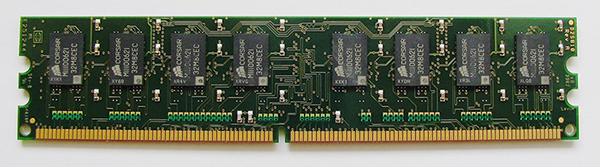
\includegraphics[width=1\textwidth]{figuress/DRAM.jpg}}
  \caption{Ini adalah DRAM}
  \label{DRAM}
  \end{figures}

1.DRAM (Dynamic RAM) adalah jenis RAM harus sering di refresh oleh CPU agar data yang terkandung didalamnya tidak hilang.
  Gambar DRAM \ref{DRAM}
  \subsection{Kelebihan dan kekurangan}
    \subsubsection{Kelebihan}
    \-Harganya lebih murah dan mengkonsumsi sedikit tenaga listrik
    \subsubsection{kekurangan}
    \-Untuk mempertahankan informasi yang disimpannya, secara periodic
    
  \begin{figures}[ht]
  \centerline{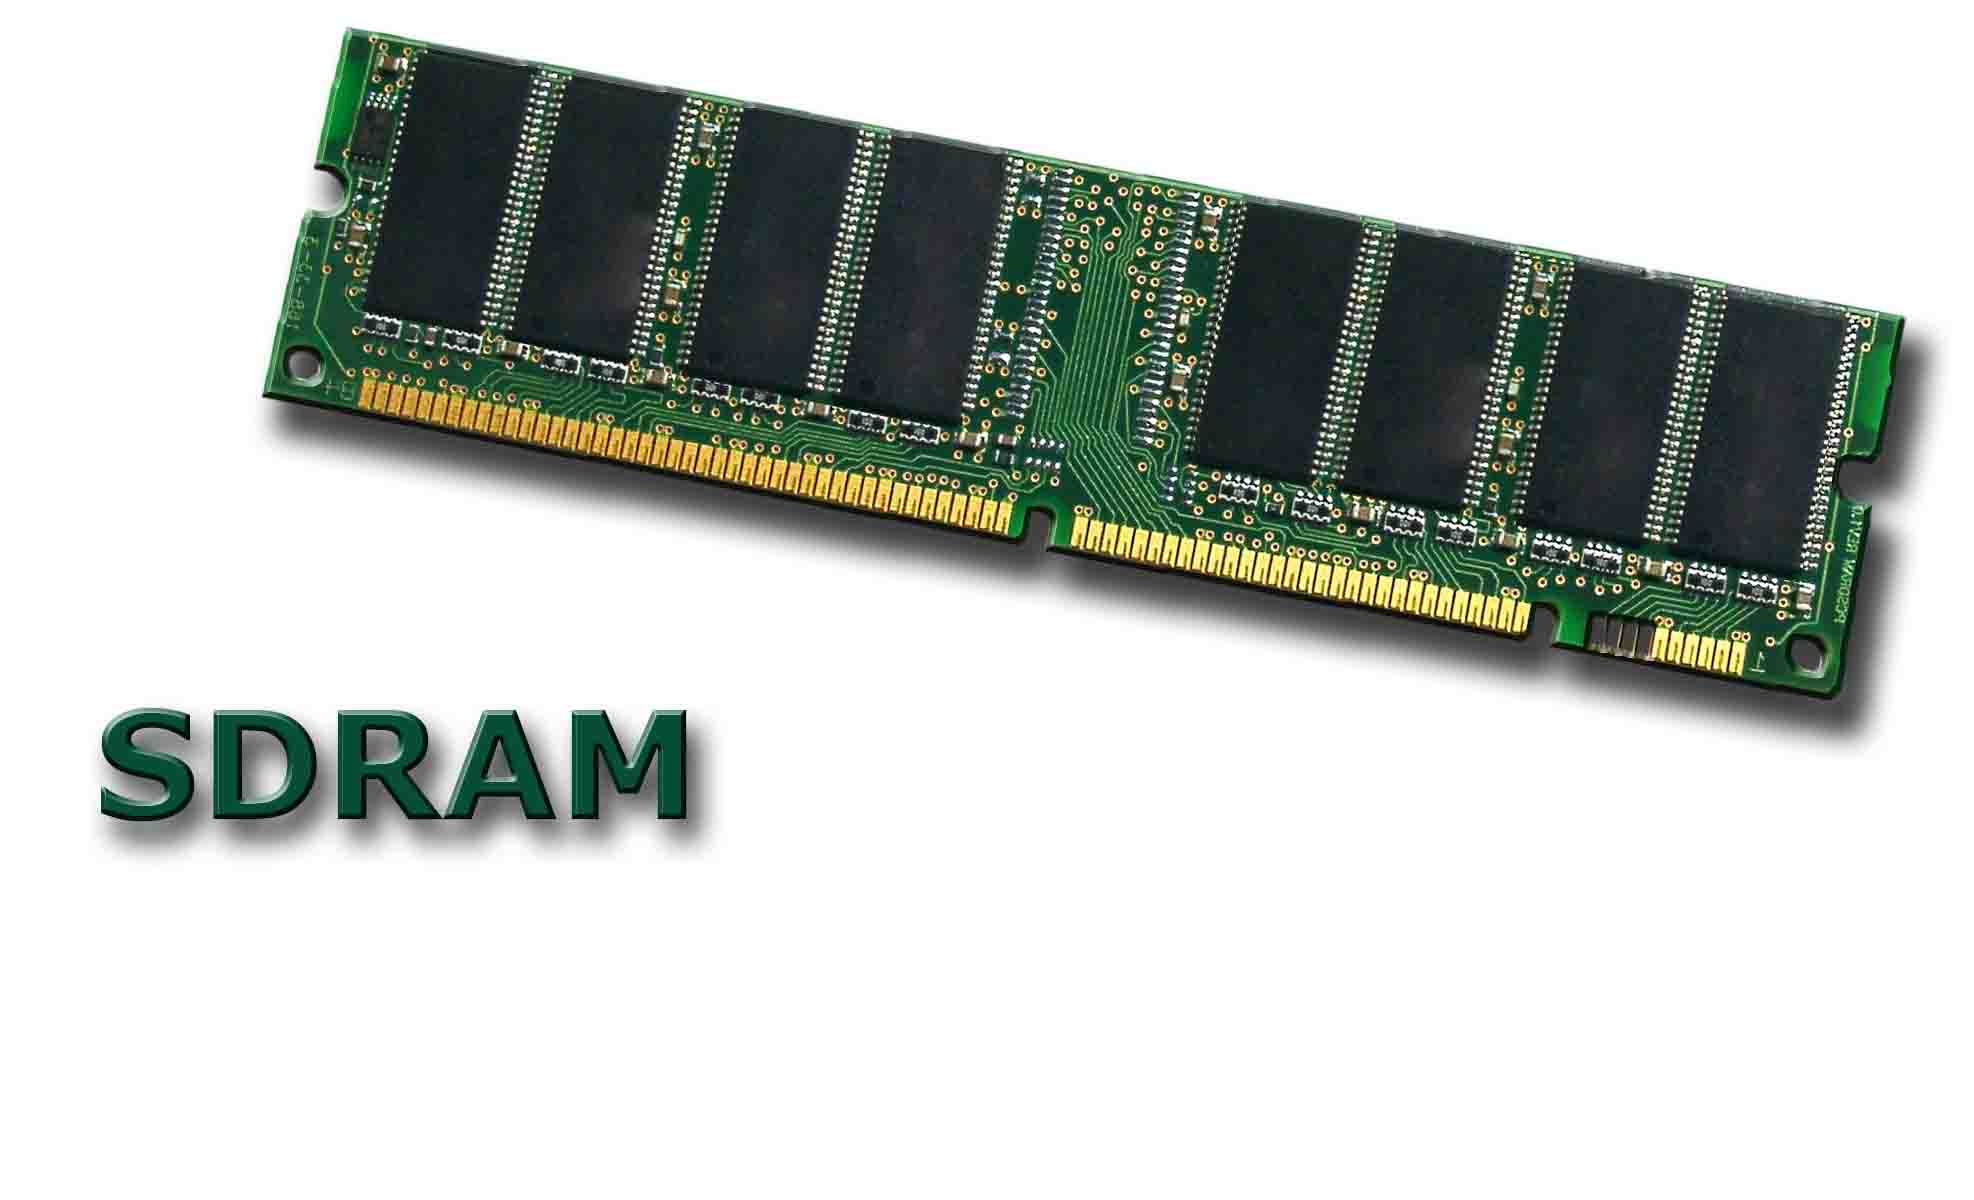
\includegraphics[width=1\textwidth]{figuress/SDRAM.jpg}}
  \caption{Ini adalah SDRAM}
  \label{SDRAM}
  \end{figures}

2.SDRAM (Synchronous Dynamic RAM) adalah jenis RAM yang paling umum digunakan pada komputer dan leptop masa sekarang. RAM ini disinkronisasi oleh clocking sistem dan memiliki kecepatan lebih tanggi dari pada DRAM serta dapat digunakan teritama dalam cache.
Gambar SDRAM \ref{SDRAM}
    \subsection{Kelebihan dan kekurangan}
    \subsubsection{Kelebihan}
    \-Memory jenis ini bisa mampu melakukan transper rate hingga 100 Mhz
    \subsubsection{kekurangan}
    \-Memory jenis ini cukup mahal

  \begin{figures}[ht]
  \centerline{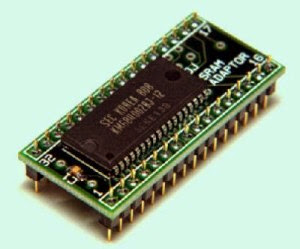
\includegraphics[width=1\textwidth]{figuress/SRAM.jpg}}
  \caption{Ini adalah SRAM}
  \label{SRAM}
  \end{figures}

3.SRAM (Statik RAM) adalah jenis memory yang tidak perlu di refresh oleh CPU supaya data yang terdapat didalamnya tetap tersimpan dengan baik.
RAM jenis ini secara bisa mempertahankan isinya selama ada listrik atau tenaga.
Gambar SRAM \ref{SRAM}
  \subsection{Kelebihan dan kekurangan}
    \subsubsection{Kelebihan}
    \-Tidak memerlukan refresh terhadap isinya dalam waktu yang cepat.
    \subsubsection{kekurangan}
    \-Harganya cukup mahal dan membutuhkan tenaga listrik yang lebih besar.

  \begin{figures}[ht]
  \centerline{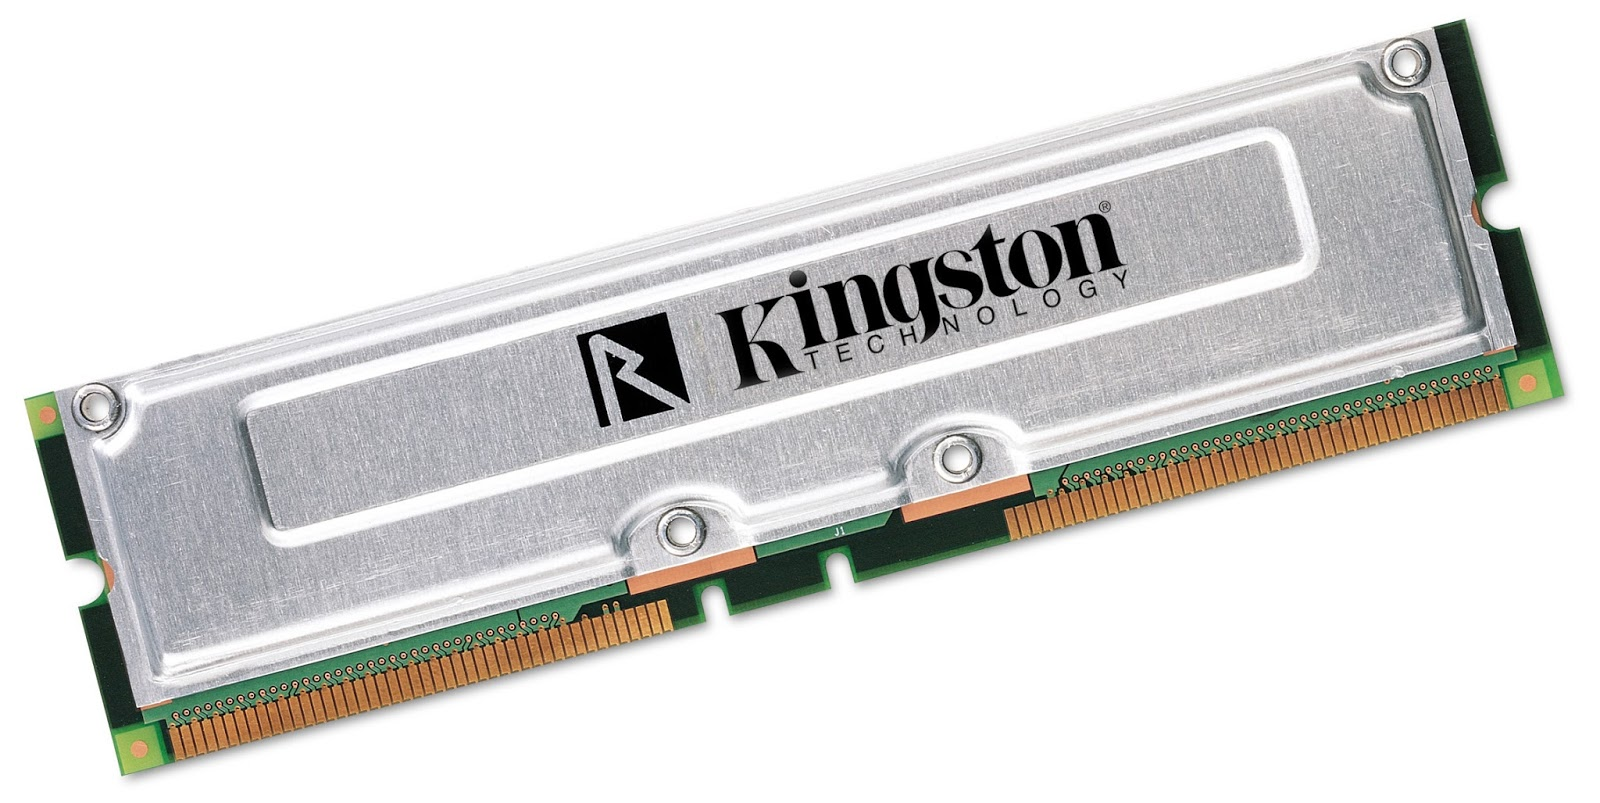
\includegraphics[width=1\textwidth]{figuress/rdram.jpg}}
  \caption{Ini adalah rdram}
  \label{rdram}
  \end{figures}

4.RDRAM (Rambus Dynamic RAM) adalah Memory yang bisa digunakan pada sistem yang menggunakan Pentium 4
Gambar RDRAM \ref{rdram}
  \subsaction{Kelebihan dan kekurangan}
    \subsubsaction{Kelebihan}
    \-Memory ini lebih cepat dari memory SDRAM
    \subsubsaction{Kekurangan}
    \-Memory ini juga memiliki kekurangan yaitu harganya lebih mahal dibandingkan dengan memory SDRAM

  \begin{figures}[ht]
  \centerline{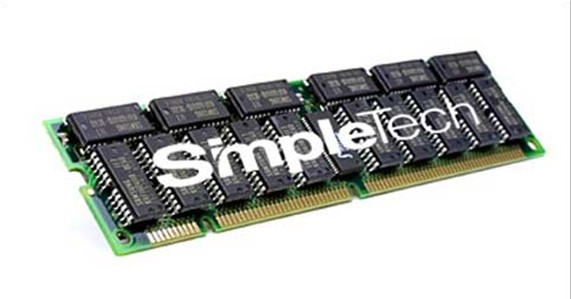
\includegraphics[width=1\textwidth]{figuress/FPMDRAM.jpg}}
  \caption{Ini adalah FPMDRAM}
  \label{FPMDRAM}
  \end{figures}

5.FPM DRAM (Fast Page Mode DRAM) adalah merupakan bentuk asli dari DRAM. Laju transfer maksimum untuk cache L2 mendekati 176 MB per sekon
Gambar FRM DRAM \ref{FPMDRAM}
  \subsaction{Kelebihan dan kekurangan}
    \subsubsaction{Kelebihan}
    \-kcepatannya cukup dinamis
    \subsubsaction{Kekurangan}
    \-Memory jenis ini membutuhkan daya yang besar
}


  \begin{figures}[ht]
  \centerline{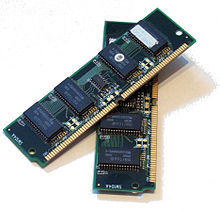
\includegraphics[width=1\textwidth]{figuress/EDODRAM.jpg}}
  \caption{Ini adalah EDODRAM}
  \label{EDODRAM}
  \end{figures}

6.EDO DRAM (Extented Data Out DRAM) adalah memory ini 5\% lebih cepat dibandingkan dengan FPM. Laju transfer maksimum untuk cache L2 mendekati 264 MB per sekon.
Gambar EDO DRAM \ref{EDODRAM}
  \subsaction{Kelebihan dan kekurangan}
    \subsubsaction{Kelebihan}
    \-Memory ini lebih cepat dibandingan dengan mmemory FRM DRAM
    \subsubsaction{Kekurangan}
    \-Memory ini cukup mahal pada masanya


  \begin{figures}[ht]
  \centerline{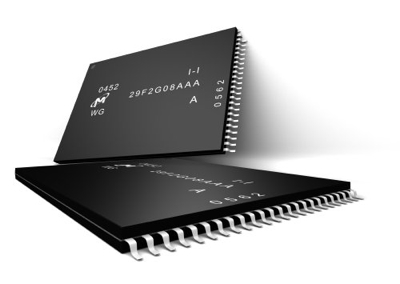
\includegraphics[width=1\textwidth]{figuress/Flashram.jpg}}
  \caption{Ini adalah Flashram}
  \label{Flashram}
  \end{figures}

7.FlashRAM adalah chip memory yang biasanya hanya terdapat pada peralatan elektronika dan tergolong memiliki kapasitas yang tergolong rendah.
Gambar FlashRAM \ref{Flashram}
  \subsaction{Kelebihan dan kekurangan}
    \subsubsaction{Kelebihan}
    \-Memiliki transper rate yang cukup
    \subsubsaction{Kekurangan}
    \-Mempertahakan informasi yang ada didalamnya

Dalam suatu artikel menyebutkan jenis \- jenis ram \cite{bruce1999unified}

\section{Kesimpulan}
Jadi menurut artikel yang telah kelompok kami buat dan kerjakan kita dapat mengetahui bahwa RAM atau Random Acces Memory itu diciptakan oleh seseorang yang bernama Robert Dennard.Random Access Memory atau yang sering kita RAM ini biasanya terdapat pada komputer digital dan Gadget anda adalah suatu tipe penyimpanan yang dapat di akses dalam waktu tetap. Dan RAM ini sudah ada sejak tahun 1960 an dan di perkenal kan oleh Robert Dennard dan telah melalui evolusi pembaruan yang sangat panjang banyak dan sangat beragam seperti RAM, FPM RAM, EDO RAM, SDM RAM hingga DDR3 RAM. Dan juga memiliki banyak jenis seperti DRAM, SDRAM, dan juga SRAM.